\documentclass[a4paper,titlepage,11pt,twosides,floatssmall]{mwrep}
\usepackage[left=2.5cm,right=2.5cm,top=2.5cm,bottom=2.5cm]{geometry}
\usepackage[OT1]{fontenc}
\usepackage{amsmath}
\usepackage{mathtools}
\usepackage{amsfonts}
\usepackage{rotating}
\usepackage{amssymb}
\usepackage{graphicx}
\usepackage{url}
\usepackage{tikz}
\usetikzlibrary{arrows,calc,decorations.markings,math,arrows.meta}
\usepackage{rotating}
\usepackage[percent]{overpic}
\usepackage[utf8]{inputenc}
\usepackage[english]{babel}
\usepackage{minted}
\usepackage{xcolor}
\usepackage{pgfplots}
\usetikzlibrary{pgfplots.groupplots}
\usepackage{listings}
\usepackage{matlab-prettifier}
\usepackage{enumitem,amssymb}
\definecolor{szary}{rgb}{0.95,0.95,0.95}
\usepackage{siunitx}
%\usepackage{tocloft} % nigdy wiecej
%\usepackage[nottoc]{tocbibind} % nigdy wiecej
\usepackage{float}
\sisetup{detect-weight,exponent-product=\cdot,output-decimal-marker={,},per-mode=symbol,binary-units=true,range-phrase={-},range-units=single}
\SendSettingsToPgf

\lstset{
	backgroundcolor=\color{szary},
	frame=single,
	breaklines=true,
}
\lstdefinestyle{customlatex}{
	basicstyle=\footnotesize\ttfamily,
	%basicstyle=\small\ttfamily,
}
\lstdefinestyle{customc}{
	breaklines=true,
	frame=tb,
	language=C,
	xleftmargin=0pt,
	showstringspaces=false,
	basicstyle=\small\ttfamily,
	keywordstyle=\bfseries\color{green!40!black},
	commentstyle=\itshape\color{purple!40!black},
	identifierstyle=\color{blue},
	stringstyle=\color{orange},
}
\lstdefinestyle{custommatlab}{
	captionpos=t,
	breaklines=true,
	frame=tb,
	xleftmargin=0pt,
	language=matlab,
	showstringspaces=false,
	%basicstyle=\footnotesize\ttfamily,
	basicstyle=\scriptsize\ttfamily,
	keywordstyle=\bfseries\color{green!40!black},
	commentstyle=\itshape\color{purple!40!black},
	identifierstyle=\color{blue},
	stringstyle=\color{orange},
}

\textwidth 160mm \textheight 247mm

\pgfplotsset{
	tick label style={font=\scriptsize},
	label style={font=\small},
	legend style={font=\small},
	title style={font=\small}
}

\def\figurename{Fig.}
\def\tablename{Tab.}

\setcounter{topnumber}{0}%2
\setcounter{bottomnumber}{3}%1
\setcounter{totalnumber}{5}%3
\renewcommand{\textfraction}{0.01}%0.2
\renewcommand{\topfraction}{0.95}%0.7
\renewcommand{\bottomfraction}{0.95}%0.3
\renewcommand{\floatpagefraction}{0.35}%0.5


\begin{document}
	
	\frenchspacing
	\makeatletter
	\def\ps@uheadings{%
		\let\@mkboth\markboth
		\let\ps@normal\hf@uheadings
		\let\ps@opening\hf@plain
		\let\ps@closing\hf@uheadings
		\let\ps@blank\hf@empty
		\ps@normal
		\def\chaptermark##1{%
			\markright{%
				\ifHeadingNumbered
				\thechapter.\enspace
				\fi
				##1}}}
	
	\pagestyle{uheadings}
	
	%strona tytułowa
	\title{\bf Altera Cyclon V Lab1 Report\vskip 0.1cm}
	\author{Jakub Wieczorek \\ Jon Märki}

	\date{2020}
	
	\makeatletter
	\renewcommand{\maketitle}{\begin{titlepage}
			\begin{center}{\LARGE {\bf
						School of Engineering}}\\
				\vspace{0.4cm}
				{\LARGE {\bf École polytechnique fédérale de Lausanne (EPFL)}}\\
				\vspace{0.3cm}
			\end{center}
			\vspace{5cm}
			\begin{center}
				{\bf \LARGE Real-Time Embedded Systems\vskip 0.1cm}
			\end{center}
			\vspace{1cm}
			\begin{center}
				{\bf \LARGE \@title}
			\end{center}
			\vspace{2cm}
			\begin{center}
				{\bf \Large \@author \par}
			\end{center}
			\vspace*{\stretch{6}}
			\begin{center}
				\bf{\large{Lausanne, \@date\vskip 0.1cm}}
			\end{center}
		\end{titlepage}
	}

	\makeatother
	
	\newcommand{\at}[2][]{#1|_{#2}}
	
	\maketitle
	
	\tableofcontents
	\setcounter{page}{2}
	\chapter{Introduction}
The goal of this project is to get in-depth knowledge in the various timings involved in interrupt handling basing on \verb|Cyclon| \verb|V| \verb|FPGA| \verb|SoC|. To achieve this, the latency of interrupt generation and interrupt handling will be measured. Specific interrupts will be generated periodically using designed timer.  
\section{Task specification}
Project consists of several parts which can be mainly divided into hardware, which is a design of \verb|SoC| done in \verb|FPGA| using \verb|Quartus| \verb|IDE| and software part, that is program in \verb|C| generating periodically interrupts. 

\begingroup
\renewcommand{\cleardoublepage}{}
\renewcommand{\clearpage}{}
\chapter{Hardware}
\endgroup
For a hardware part \verb|Quartus| \verb|IDE| was exploited. First part consists of a system configuration. \verb|SoC| has to be built from already designed components which are processor, memory and JTAG, they are respectively \verb|NIOS II|, 256kB  \verb|On-Chip| \verb|Memory| and \verb|JTAG| \verb|UART| -- to see the results on the screen. When above components are connected to one another, clocks, reset signals are tracked to proper pins, the next part is to write in \verb|VHDL| custom counter which will measure the time interrupt handling and parallel port to communicate with the system in parallel. Both of them has to be realised as an independent \verb|Qsys| components, therefore they have to communicate using specific \verb|Altera| bus -- \verb|Avalon|. Component means black box with pins opened for the outer world. Then user can simple take ready component and pick him up for his system without consciousness how is he working inside. 

\subsection{Avalon Bus}
\verb|Avalon| bus is a mediator with the processor and different \verb|SoC| components. As a consequence they have to follow \verb|Avalon| signal's convention.

\begin{minted}{vhdl}
ENTITY avalon_bus IS
    PORT
    (
        Clk         : IN  std_logic;
        nReset      : IN  std_logic;
        Address     : IN  std_logic_vector (2 DOWNTO 0);
        ChipSelect  : IN  std_logic;
        Read        : IN  std_logic;
        Write       : IN  std_logic;
        ReadData    : OUT std_logic_vector (31 DOWNTO 0);
        WriteData   : IN  std_logic_vector (31 DOWNTO 0)
    );
END ENTITY;
\end{minted}

\verb|Clk| and \verb|nReset| ale clock and reset signals, where the second one is negated -- high when zero. \verb|Address| is a control signal. Depending on his value different operation are performed, that is for example start counter, stop him or write to the parallel port, here his length is 3, but can be extended without any problems. If \verb|ChipSelect| is 1, then specifically that component is chosen to communicate. \verb|Read|, \verb|Write| are set when respectively system wants read values from component -- precisely from \verb|ReadData| or write them to the system -- precisely component will read them from \verb|WriteData| vector. For example to start counter \verb|ChipSelect|, \verb|Write| have to be set high and proper control value set in \verb|Address| signal.

\section{Counter} \label{sec:counter}
Counter is characterised by the following features:
\begin{enumerate}
  \item 32-bit Avalon slave
  \item 32-bit counter
  \item 1 wait cycle for read access (synchronous read)
  \item Increment the counter at the system's clock speed 50MHz
  \item Command to reset the counter, start and stop the counter
  \item The counter value must be available to read all the time -- transfer the counter value at the start of the read clock cycle.
\end{enumerate}

\subsection{Implementation}
First of all counter has signals to communicate using \verb|Avalon bus|. Additionally he has interrupt signal, which will be fired when counter reaches zero. 


\begin{minted}{vhdl}
ENTITY counter IS
    PORT
    (
        -- Avalon signals
        IRQ : out STD_LOGIC
    );
END ENTITY;
\end{minted}
Additionally he has several inner signals like counter variable, enable, reset and signals responsible for interrupt.
\begin{minted}{vhdl}
signal iCounter : unsigned(31 DOWNTO 0);
signal iEn      : std_logic; -- stop/start
signal iRz      : std_logic; -- reset counter
signal iEOT     : std_logic; -- '1' when counter equals 0
signal iClrEOT  : std_logic; -- clear equals zero flag
signal iIRQEn   : std_logic;
\end{minted}
\verb|iCounter| is increased as long as \verb|iEn| is set. \verb|iEn| and \verb|iRz| are controlled by \verb|Avalon's| signal \verb|Address|. When counter reaches zero, then \verb|iEOT| is set. That signal can be later on cleared when \verb|iClrEOT| is set and will be set when proper manipulation on \verb|Avalon's| signal are performed. Similarly to \verb|iIRQEn|.

Counter consists of several processes which are ran in parallel according to \verb|FPGA| architecture. First of them counter process which increases \verb|iCounter| signal in every clock cycle unless \verb|iRz| is not set and counter is not stopped. 

\begin{minted}{vhdl}
pCounter : process(Clk) begin
    if rising_edge(Clk) then
        if iRz= '1' then
            iCounter <= (others => '0');
        elsif iEn = '1' then
            iCounter <= iCounter+1;
        end if;
    end if;
end process pCounter;
\end{minted}
Next process is responsible for writing to the counter. When processor wants to talk to that component he has to pull his \verb|ChipSelect| signal high, pull also \verb|write| signal high and set proper value in \verb|Address| control register. It is worth to notice that the last two inner signals are set or reset according to the first bit in \verb|WriteData| vector.
\begin{minted}{vhdl}
pRegWr : process(Clk, nReset) begin
    if nReset = '0' then 
        iEn     <= '0'; 
        iRz     <= '0';
        iIRQEn  <= '0';
    elsif rising_edge(Clk) then
        iRz     <= '0';
        iClrEOT <= '0';
        
        if ChipSelect = '1' and Write = '1' then -- Write cycle
            case Address(2 downto 0) is
                when "001" => iRz       <= '1'; -- Reset Counter (pulse)
                when "010" => iEn       <= '1'; -- Start Run
                when "011" => iEn       <= '0'; -- Stop Run
                when "100" => iIRQEn    <= WriteData(0);
                when "101" => iClrEOT   <= WriteData(0);
                when others => null;
            end case;
        end if;
    end if;
end process pRegWr;
\end{minted}
The same with the fallowing process, but in this case he is responsible for reading values from the component instead of writing to. In that way counter value can be read in the next clock cycle according to the task specification as well as check if counter is running or not and if the zero flag is set or not. Also whether interrupt is enabled can be checked. 

\begin{minted}{vhdl}
pRegRd : process(Clk) begin -- Read cycle
    if rising_edge(Clk) then
        ReadData <= (others => '0'); -- default value
            if ChipSelect = '1' and Read = '1' then -- Read cycle
                case Address(2 downto 0) is
                when "000"  => ReadData     <= std_logic_vector(iCounter);
                when "100"  => ReadData(0)  <= iIRQEn;
                when "101"  => ReadData(0)  <= iEOT;
                               ReadData(1)  <= iEn; -- Run
                when others => null;
            end case;
        end if;
    end if;
end process pRegRd;
\end{minted}
Last two processes are responsible for interrupts. Interrupt is fired only when counter reaches zero, so \verb|iEOT| flag is set, interrupts are enabled and counter is running.
\begin{minted}{vhdl}
pInterrupt : process(Clk) begin
    if rising_edge(Clk) then
        if iCounter = X"0000_0000" then
            iEOT <= '1';
        elsif iClrEOT = '1' then
            iEOT <= '0';
        end if;
    end if;
end process pInterrupt;

IRQ <= '1' when iEOT = '1' and iIRQEn = '1' and iEn = '1' else '0';
\end{minted}

\subsection{Testing}
To verify the design, test bench was written what allows to look at the waveform for every signal and check if implementation is correct or not. To test the design \verb|ModelSim| software was exploited. On the following code listing the test bench is presented. It is normal \verb|.vhd| file with empty \verb|Entity|, which uses \verb|Counter| design unit as a component and manipulates his signals -- \verb|Avalon| bus. Clock cycle is set to 10ns. 
\begin{minted}{vhdl}
constant clk_period : time := 10 ns;
\end{minted}
And process responsible for clock manipulation. 
\begin{minted}{vhdl}
clk_process : process begin
    Clk <= '1';
    wait for clk_period/2;
    Clk <= '0';
    wait for clk_period/2;
end process clk_process;
\end{minted}
Chip select is pulled up all the time.
\begin{minted}{vhdl}
ChipSelect <= '0', '1' after clk_period*2;
\end{minted}
Simulation is terminated after 100 clock cycles.
\begin{minted}{vhdl}
stop_sim : process begin
    wait for clk_period * 100;
    assert false;
    report "simulation finished" severity failure;
end process stop_sim;
\end{minted}

\figurename{} \ref{fig:counter_read_latency} shows a piece of a wave form where yellow marker points for a one clock delay according to the task specification between \verb|iCounter| and \verb|ReadData|.

\begin{figure}[H]
	\begin{center}
		\scalebox{0.5}{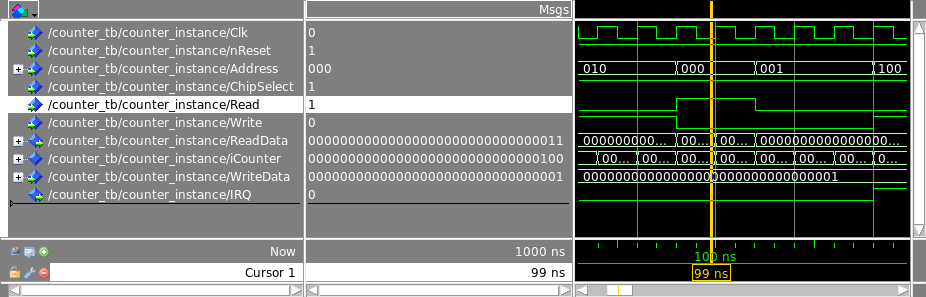
\includegraphics{./pictures/counter_read_latency.png}}
	\end{center}
	\caption{One clock cycle latency for counter read}
	\label{fig:counter_read_latency}
\end{figure}

Additionally from counter design the component was created using \verb|Qsys| software. That component is ready to be copied  to any different project. It is like a black box with closed and thoroughly tested logic. Counter component can be seen at the \figurename{} \ref{fig:interrupt_counter_component}. Subsequently it was added to the system and connected with clock, reset\_sink, interrupt\_sender and avalon\_slave\_0 and an memory slave.

\begin{figure}[H]
	\begin{center}
		\scalebox{1}{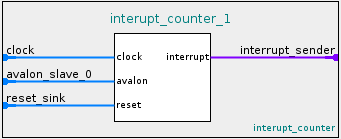
\includegraphics{./pictures/interrupt_counter_component.png}}
	\end{center}
	\caption{Counter component}
	\label{fig:interrupt_counter_component}
\end{figure}

\section{Parallel port}
Parallel port is a mediator in communication between system components and the outer world for example LEDs or buttons. 

\subsection{Implementation}
Apart from \verb|Avalon| signals which are exactly the same as for \verb|Counter| one more signal is defined. That is a vector of generic length up to 32 bits. 
\begin{minted}{vhdl}
ENTITY parallel_port is 
    GENERIC(N : integer);
    PORT
    (
        -- avalon bus
        ParPort : inout std_logic_vector(N-1 downto 0)
    );
END parallel_port;
\end{minted}
This vector is a bidirectional parallel port where, every single bit can be configured as an input or an output. Three inner signals where declared to keep the direction, current state of parallel port and data.
\begin{minted}{vhdl}
signal iRegDir : std_logic_vector (N-1 DOWNTO 0); -- direction
signal iRegPort: std_logic_vector (N-1 DOWNTO 0); -- data register 
signal iRegPin : std_logic_vector (N-1 DOWNTO 0); -- current pin state
\end{minted}
\verb|iRegDir| is a direction register, when a bit in that register is set to 1 then it is output otherwise it is input. For every particular bit in \verb|iRegDir| set to 1 corresponding bit in \verb|iRegPort| will be assigned to the \verb|ParPort|, for every 0 it will be high impedance Z state.
\begin{minted}{vhdl}
pPort : process(iRegDir, iRegPort) -- direction process
begin
    for i in 0 to N-1 loop
        if iRegDir(i) = '1' then
            ParPort(i) <= iRegPort(i); -- write
        else
            ParPort(i) <= 'Z'; -- read
        end if;
    end loop;
end process pPort;
\end{minted}
Process responsible for a direction configuration and data copying from \verb|WriteData| vector to the inner register \verb|iRegPort| is shown below.
\begin{minted}{vhdl}
pRegWr : process(Clk, nReset) -- write (control) process (to the port)
begin
    if nReset = '0' then
        iRegDir <= (others => '0'); -- Input by default
    elsif rising_edge(Clk) then
        if ChipSelect = '1' and Write = '1' then -- Write cycle
            case Address(2 downto 0) is
            when "000" => iRegDir   <= WriteData(N-1 downto 0); -- control direction
            when "010" => iRegPort  <= WriteData(N-1 downto 0); -- write data
            when "011" => iRegPort  <= iRegPort OR WriteData(N-1 downto 0);
            when "100" => iRegPort  <= iRegPort NAND WriteData(N-1 downto 0);
            when others => null;
            end case;
        end if;
    end if;
end process pRegWr;
\end{minted}
Similarly to \verb|Counter| component here \verb|Address| indicates what is inside \verb|WriteData| (data or direction) or what operation are to be done on the \verb|iRegPort| register. 

Value of a \verb|PortMap| is all the time accessible in \verb|iRegPin| register.
\begin{minted}{vhdl}
iRegPin <= ParPort;
\end{minted}
Of course he has to be read using \verb|Avalon| interface. Following process is responsible for that.
\begin{minted}{vhdl}
pRegRd : process(Clk) -- read process
begin
    if rising_edge(Clk) then
        ReadData <= (others => '0'); -- zeros by default
            if ChipSelect = '1' and Read = '1' then -- Read cycle
            case Address(2 downto 0) is
                when "000"  => ReadData(N-1 downto 0) <= iRegDir;
                when "001"  => ReadData(N-1 downto 0) <= iRegPin;
                when "010"  => ReadData(N-1 downto 0) <= iRegPort;
                when others => null;
            end case;
        end if;
    end if;
end process pRegRd;
\end{minted}
\subsection{Testing}
To test the design one test bench was created. Writing as well as reading was tested. In the test bench the generic size of the port was set to 8 bits. At the beginning of the test the direction was set by \verb|Address| = "000", \verb|Write| = "1" and \verb|WriteData| = "... 11110001". The waveform from that part can be observed on the \figurename{} \ref{fig:parallel_direction}.
\begin{figure}[H]
	\begin{center}
		\scalebox{0.4}{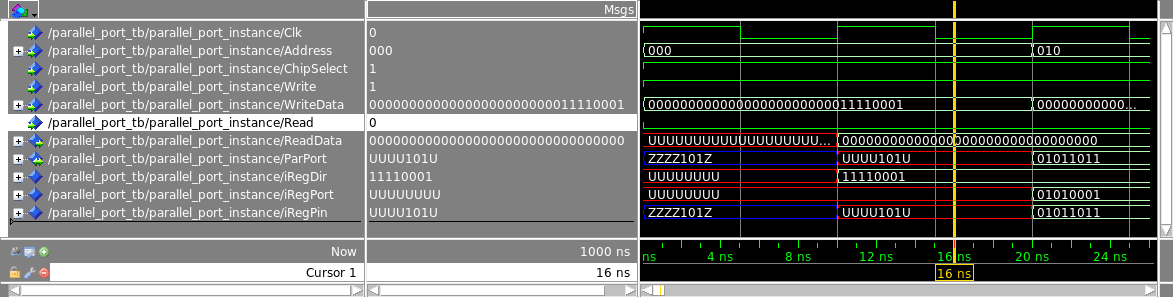
\includegraphics{./pictures/parallel_direction.png}}
	\end{center}
	\caption{Direction manipulation on the parallel port. Waveform}
	\label{fig:parallel_direction}
\end{figure}

In the next clock cycle data were sent \verb|WriteData| = "... 01010001". Waveform is shown on the 
\figurename{} \ref{fig:parallel_data_write}.
\begin{figure}[H]
	\begin{center}
		\scalebox{0.4}{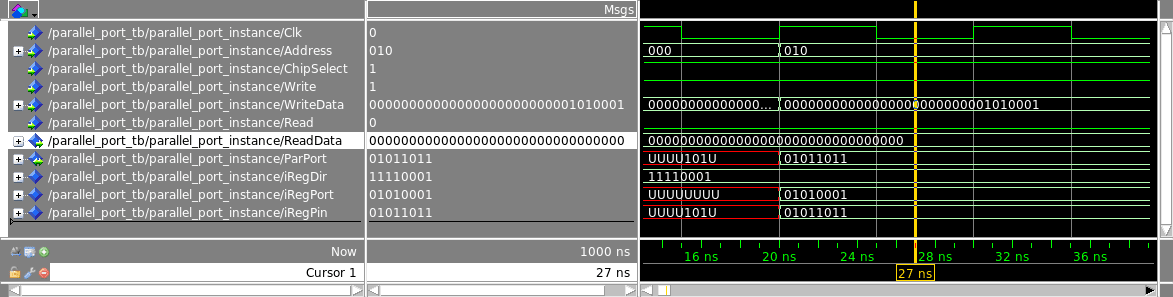
\includegraphics{./pictures/parallel_data_write.png}}
	\end{center}
	\caption{Direction manipulation on the parallel port. Waveform}
	\label{fig:parallel_data_write}
\end{figure}

Next clock cycle is for reading the data from \verb|ParPort|. At the beginning of the test \verb|ParPort| was set to "ZZZZ101Z", it means with the connection with the direction that "01011011" should be visible in the \verb|iRegPin|, and after the read cycle should be visible in the \verb|ReadData| vector.
Waveform is shown on the 
\figurename{} \ref{fig:parallel_data_read}.
\begin{figure}[H]
	\begin{center}
		\scalebox{0.4}{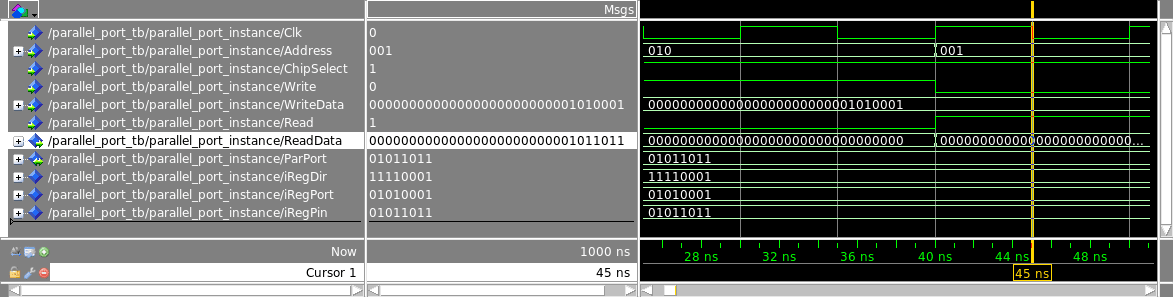
\includegraphics{./pictures/parallel_data_read.png}}
	\end{center}
	\caption{Direction manipulation on the parallel port. Waveform}
	\label{fig:parallel_data_read}
\end{figure}

Additionally from parallel design the component was created using \verb|Qsys| software -- similarly to the counter component. Parallel component can be seen at the \figurename{} \ref{fig:parallel_port_component}. Subsequently it was added to the system and connected with clock, reset\_sink and avalon\_slave\_0 and an memory slave. \verb|Parallel_port| bidirectional vector was done as a \verb|Conduit|, that is interface for an I/O connections and exported as an external connection. 

\begin{figure}[H]
	\begin{center}
		\scalebox{1}{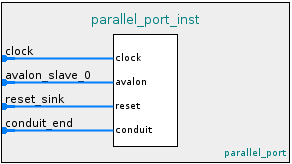
\includegraphics{./pictures/parallel_port_component.png}}
	\end{center}
	\caption{Parallel port component}
	\label{fig:parallel_port_component}
\end{figure}

\subsection{Full design}
Finally the \verb|SoC| design consists of two created components connected with \verb|Nios| processor, \verb|SDRAM| controller, \verb|JTAG|, \verb|LEDs|, buttons, \verb|PLL| loop frequency multiplier and \verb|GPIO| pins connected to the parallel port. All connections between particular components are presented on the \figurename{} \ref{fig:soc_system}.

\begin{figure}[H]
	\begin{center}
		\scalebox{0.35}{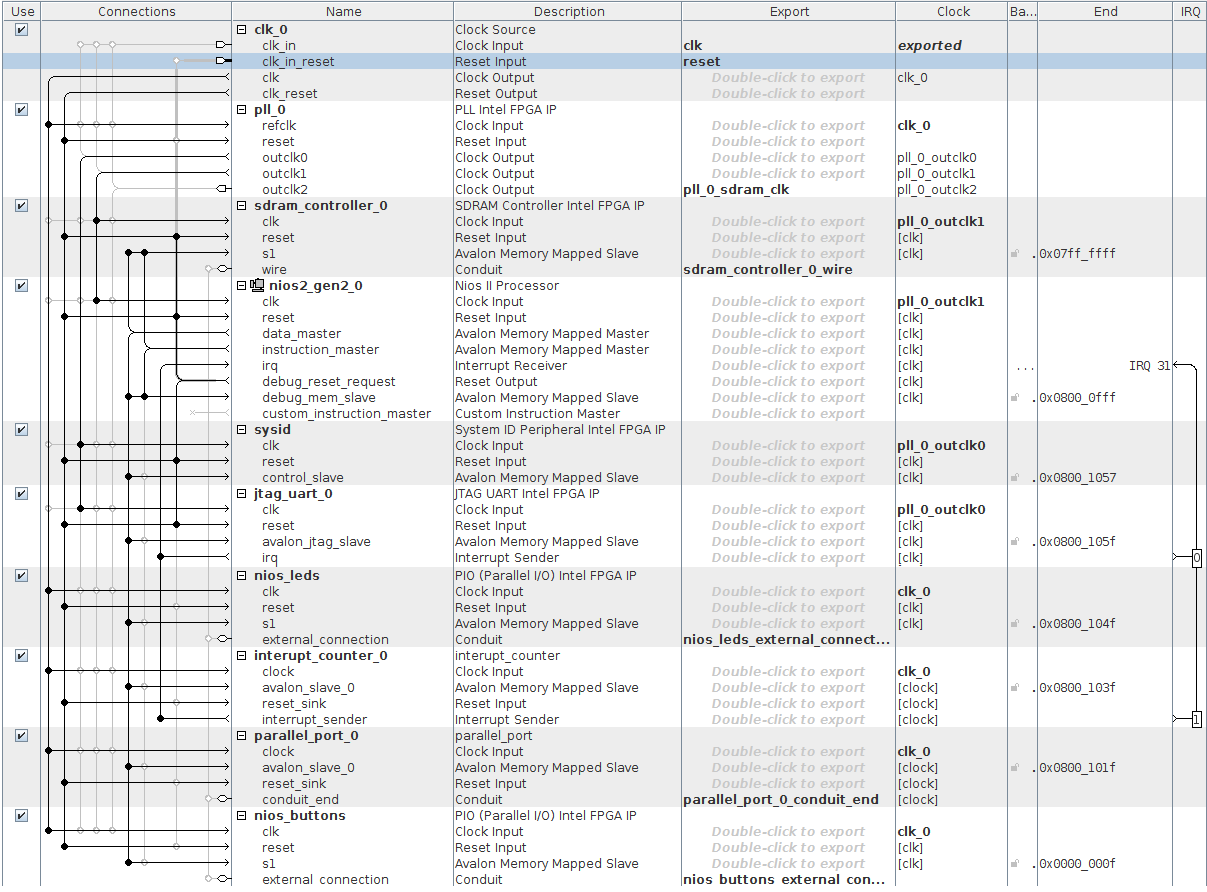
\includegraphics{./pictures/soc_system.png}}
	\end{center}
	\caption{SoC design connections}
	\label{fig:soc_system}
\end{figure}

Additionally to \verb|Qsis| design showed on \figurename{} \ref{fig:soc_system} it is necessary to connect \verb|SDRAM|, parallel port, clk, reset leds, buttons and pll with real physical pins and connection inside the chip \verb|Cyclon V|. To do that in the top module system component was created and instantiated. On the fallowing listing \verb|entity| with real pins was presented.

\begin{minted}{vhdl}
entity DE1_SoC_top_level is
    port
    (
        CLOCK_50    : in    std_logic;
        
        -- KEY_n
        KEY_N       : in    std_logic_vector(3 downto 0);
        
        -- LED
        LEDR        : out   std_logic_vector(9 downto 0);
        
        -- SDRAM
        DRAM_ADDR   : out   std_logic_vector(12 downto 0);
        DRAM_BA     : out   std_logic_vector(1 downto 0);
        DRAM_CAS_N  : out   std_logic;
        DRAM_CKE    : out   std_logic;
        DRAM_CLK    : out   std_logic;
        DRAM_CS_N   : out   std_logic;
        DRAM_DQ     : inout std_logic_vector(15 downto 0);
        DRAM_LDQM   : out   std_logic;
        DRAM_RAS_N  : out   std_logic;
        DRAM_UDQM   : out   std_logic;
        DRAM_WE_N   : out   std_logic;
        
        -- GPIO_0
        GPIO_0      : inout std_logic_vector(35 downto 0)
    );
end DE1_SoC_top_level;
\end{minted}
Subsequently the component declaration.
\begin{minted}{vhdl}
component soc_system is
port (
clk_clk                 : in    std_logic                     := 'X';
reset_reset_n           : in    std_logic                     := 'X';
reset_n
sdram_controller_0_wire_addr            : out   std_logic_vector(12 downto 0);                    
sdram_controller_0_wire_ba              : out   std_logic_vector(1 downto 0);                     
sdram_controller_0_wire_cas_n           : out   std_logic;
sdram_controller_0_wire_cke             : out   std_logic;
sdram_controller_0_wire_cs_n            : out   std_logic;
sdram_controller_0_wire_dq    : inout std_logic_vector(15 downto 0) := (others => 'X');
sdram_controller_0_wire_dqm   : out   std_logic_vector(1 downto 0);
sdram_controller_0_wire_ras_n           : out   std_logic;
sdram_controller_0_wire_we_n            : out   std_logic;
parallel_port_0_conduit_end_export : inout std_logic_vector(31 downto 0) := (others => 'X');
nios_leds_external_connection_export    : out   std_logic_vector(9 downto 0);
pll_0_sdram_clk_clk                     : out   std_logic;
nios_buttons_external_connection_export : in std_logic_vector(2 downto 0) := (others => 'X')
);
end component;
\end{minted}
And component instantiation.
\begin{minted}{vhdl}
u0 : soc_system
	port map (
		clk_clk                                 => CLOCK_50,
		reset_reset_n                           => KEY_N(0), 
		sdram_controller_0_wire_addr            => DRAM_ADDR,
		sdram_controller_0_wire_ba              => DRAM_BA,
		sdram_controller_0_wire_cas_n           => DRAM_CAS_N,
		sdram_controller_0_wire_cke             => DRAM_CKE,
		sdram_controller_0_wire_cs_n            => DRAM_CS_N,
		sdram_controller_0_wire_dq              => DRAM_DQ,
		sdram_controller_0_wire_dqm(1)          => DRAM_UDQM,
		sdram_controller_0_wire_dqm(0)          => DRAM_LDQM,
		sdram_controller_0_wire_ras_n           => DRAM_RAS_N,
		sdram_controller_0_wire_we_n            => DRAM_WE_N,
		parallel_port_0_conduit_end_export      => GPIO_0(31 DOWNTO 0),
		nios_leds_external_connection_export    => LEDR(9 DOWNTO 0),
		pll_0_sdram_clk_clk                     => DRAM_CLK,
		nios_buttons_external_connection_export => KEY_N(3 DOWNTO 1)
	);
\end{minted}

Above code basically was copied from \verb|Qsis| generated file. Now full hardware design ready to be programmed into the board was created. Next chapter focuses on the software part. It is worth to note that \verb|.tcl| script was executed in order to map all the pins from the design into those available on the \verb|DE1-SoC| board. It is necessary to connect all the pins with designed \verb|SoC| components -- the process is similar to pins mapping using \verb|user| \verb|constraints| \verb|file| known for example from \verb|Xilinx| \verb|FPGA| development. After mentioned operation with \verb|.tcl| file \verb|FPGA| is ready to be programmed by the \verb|.sof| (SRAM Object File) output file \footnote{It is necessary to load .sof file whenever board is restarted, since there can be some problems with programming the board with C program}.

\begingroup
\renewcommand{\cleardoublepage}{}
\renewcommand{\clearpage}{}
\chapter{Software}
\endgroup
The next part of the system design is software which will be running on the \verb|Nios| \verb|II| processor.

\section{Interrupts performance}
Interrupt Service Routine (ISR) performance can be measured by three fallowing metrics: interrupt latency, response time and recovery time. \verb|Interrupt| \verb|latency| is the time from when an interrupt is
first generated to when the processor runs the first
instruction at the exception address. \verb|Interrupt| \verb|response| \verb|time| is the time from when an
interrupt is first generated to when the processor runs
the first instruction in the ISR. Finally \verb|Interrupt| \verb|recovery| \verb|time| is the time taken from the last
instruction in the ISR to return to normal processing. 

\subsection{Interrupt response time}
To measure interrupt response time built-in timer was utilised. The timer is showed on the picture \ref{fig:soc_system}. To make it possible to use the driver in the software part in \verb|eclipse| it is necessary to edit \verb|BSP| settings and (\verb|settings.bsp|) and change under the \verb|hal| section \verb|sys_clk_timer| and \verb|timestamp_timer| to \verb|timer_0| -- the timer from the SoC design. By default that two fields are set to None. Once again it is very important to set time period (in \verb|qsis|) for interval timer not too low, otherwise interrupt will be triggered faster than any instruction finishes. 

The idea is to generate an interrupt periodically and measure a timer value inside an \verb|Interrupt| \verb|Service| \verb|Routine| (\verb|ISR|). When timer reaches 0 the interrupt is fired, but the timer still counts. The value of the timer inside \verb|ISR| indicates interrupt response time. Timer value can be read using snap register. Timer utilised in this paper is 32-bit length and the timer value is held in two 16-bit snap registers -- \verb|snapl| for the less significant part and \verb|snaph| for the second one. To read value from a snap register first a write operation into that register has to be performed (write-data is ignored, any value can be used). Then a timer value is copied into that register and can be accessed. The following listing shows timer configuration. 
\begin{lstlisting}[style=customc, frame=none]
void setup_response_timer()
{
    alt_ic_isr_register(TIMER_0_IRQ_INTERRUPT_CONTROLLER_ID,
    TIMER_0_IRQ,my_isr, NULL,NULL);
    flag=0;
    IOWR_ALTERA_AVALON_TIMER_CONTROL(TIMER_0_BASE,0);
    IOWR_ALTERA_AVALON_TIMER_CONTROL(TIMER_0_BASE,2);
    IOWR_ALTERA_AVALON_TIMER_PERIODL(TIMER_0_BASE, 0xFFFF); 
    IOWR_ALTERA_AVALON_TIMER_PERIODH(TIMER_0_BASE, 0x00FF);
    IOWR_ALTERA_AVALON_TIMER_CONTROL(TIMER_0_BASE,3);
    IOWR_ALTERA_AVALON_TIMER_CONTROL(TIMER_0_BASE,7);
}
\end{lstlisting}
At the beginning an \verb|ISR| has to be registered. Subsequently control register is cleared (second instruction), continues mode is set, period registers are initialised. The timer is counts downwards. Last two instructions enables timer interrupts and starts the timer. Flag is a global volatile variable and tells if interrupt occurred. Next listing shows \verb|ISR|.
\begin{lstlisting}[style=customc, frame=none]
static void my_isr(void* context)
{
    IOWR_ALTERA_AVALON_TIMER_SNAPL(TIMER_0_BASE, ARBITVAL);
    snapl = IORD_ALTERA_AVALON_TIMER_SNAPL(TIMER_0_BASE);
    snaph = IORD_ALTERA_AVALON_TIMER_SNAPH(TIMER_0_BASE);
    
    IOWR_ALTERA_AVALON_TIMER_CONTROL(TIMER_0_BASE,0);
    IOWR_ALTERA_AVALON_TIMER_STATUS(TIMER_0_BASE, 0);
    flag=1;
}
\end{lstlisting}
At the beginning as it was noted, snap register is accessed first by writing some data into him and then by reading the register into the \verb|snapl| global variable. Next the interrupt flag has to be cleared. Otherwise immediately when \verb|ISR| finishes, program will invoke him once again. 
In the main program function, timer is set-up. Then if interrupt occurred (flag variable) the snap register is printed into stdout. Finally timer interrupts are enabled once again.
\begin{lstlisting}[style=customc, frame=none]
// main.c
int main()
{
    setup_response_timer();

    while (true)
    {
        measure_response_time();
        
        usleep(SLEEP_DELAY_US);
    }
    
    return 0;
}
// inerrupt_measurement.c
void measure_response_time()
{
    if(flag)
    {
        alt_printf("response time = %x \n",0xffff-snapl+1);
        flag=0;
         //Enable IRQ and Start timer
        IOWR_ALTERA_AVALON_TIMER_CONTROL(TIMER_0_BASE,7);
    }
}
\end{lstlisting}
The interrupt response varies between while loop cycles and is between 75 and 80 cycles. Usually is 0x4b (75).

\subsection{Interrupt recovery time}
Interrupt recovery time will be measured using a timer designed as an IP component which communicates with the rest of the system according to the \verb|Avalon| bus specification. Timer can be seen on \figurename{} \ref{fig:interrupt_counter_component}. Only external pins are presented, nevertheless inside of course there are \verb|Avalon| bus connections. On the \figurename{} \ref{fig:soc_system} showed a way in which an \verb|interrupt_counter_0| is connected with the rest of a \verb|SoC| system.

First thing necessary to perform is test if it is possible to properly communicate with a timer using software, that is C code. Following code listing demonstrates counter test function which is executed in the \verb|main| procedure. Address of a counter component is stored in a  \verb|INTERRUPT_COUNTER_0_BASE| macro in \verb|bsp| library. At the beginning the counter is reset. It is worth noting, that to reset, start and stop the counter it is not important what is inside the data stream, that is why for these operations \verb|ARBITVAL| is passed as a third argument to \verb|IOWR| function. \verb|ARBITVAL| is set to 0x0000FFFF, but can be any different one. To perform 3 mentioned operations only the register value is needed -- \verb|IRZ|, \verb|ISTART|, \verb|ISTOP|, which represents an \verb|Address| signal from \verb|Avalon| bus. It is clearly visible on the counter implementation described in the section \ref{sec:counter}. 
\begin{lstlisting}[style=customc, frame=none]
#include "counter_test.h"

void test_counter()
{
    // reset
    IOWR(INTERRUPT_COUNTER_0_BASE, IRZ, ARBITVAL);
    alt_printf("iCounter after reset= %x\n", 
        IORD(INTERRUPT_COUNTER_0_BASE, ICOUNTER));
    
    //start
    IOWR(INTERRUPT_COUNTER_0_BASE, ISTART, ARBITVAL);
    alt_printf("iCounter after start= %x\n", 
        IORD(INTERRUPT_COUNTER_0_BASE, ICOUNTER));
    
    // stop two times,  should give the same result
    IOWR(INTERRUPT_COUNTER_0_BASE, ISTOP, ARBITVAL);
    alt_printf("iCounter after stop1= %x\n", 
        IORD(INTERRUPT_COUNTER_0_BASE, ICOUNTER));
    alt_printf("iCounter after stop2= %x\n", 
        IORD(INTERRUPT_COUNTER_0_BASE, ICOUNTER));
    
    // restart and read two times, should give different result
    IOWR(INTERRUPT_COUNTER_0_BASE, ISTART, ARBITVAL);
    alt_printf("iCounter after restart1=%x\n",
        IORD(INTERRUPT_COUNTER_0_BASE,ICOUNTER));
    alt_printf("iCounter after restart2=%x\n",
        IORD(INTERRUPT_COUNTER_0_BASE,ICOUNTER));
    
    IOWR(INTERRUPT_COUNTER_0_BASE, ISTOP, ARBITVAL);
}
\end{lstlisting}
The counter is first reset, launched, stopped two times to show that a value is the same between two consecutive stops and started once again. After that when the counter is running two reads are performed again, this time to prove that counter counts indeed. The macros to control the counter and the header files are showed below.
\begin{lstlisting}[style=customc, frame=none]
#include "io.h"
#include "altera_avalon_pio_regs.h"
#include "system.h"
#include "sys/alt_stdio.h"

#define ICOUNTER 0

#define IRZ 1
#define ISTART 2
#define ISTOP 3
#define IIRQEN 4
#define ICLREOT 5

#define IRQENVAL 1
#define IRQDISVAL 0
#define CLREOTVAL 1
#define ARBITVAL 0X0000FFFF
\end{lstlisting}
The result of the test is showed on the following listing.
\begin{lstlisting}[frame=single]
iCounter after reset= 0
iCounter after start= d
iCounter after stop1= 64fe
iCounter after stop2= 64fe
iCounter after restart1=6501
iCounter after restart2=d5da
\end{lstlisting}

When the counter is roughly tested, the next step is interrupt recovery time measurement. The logic behind it is very similar to response measurement, but this time, time will be measured between the last instruction in the timer \verb|ISR| and first instruction outside this interrupt handler by \verb|IP| counter component. When interrupt is triggered (timer reaches 0), then the last instruction in \verb|ISR| is \verb|interrupt_conter_0| launch. In the main function, \verb|interrupt_conter_0| value is polling all the time and checked if is different than zero, if so that value is a recovery time. The following listing shows a polling which is invoked in the main function. 
\begin{lstlisting}[style=customc, frame=none]
void measure_recovery_time()
{
    while(IORD(INTERRUPT_COUNTER_0_BASE, ICOUNTER)==0);
    alt_printf("recovery time%x \n",
        IORD(INTERRUPT_COUNTER_0_BASE, ICOUNTER));
    
    // run it again
    IOWR(INTERRUPT_COUNTER_0_BASE, ISTOP, ARBITVAL);
    IOWR(INTERRUPT_COUNTER_0_BASE, IRZ, ARBITVAL);
    IOWR_ALTERA_AVALON_TIMER_CONTROL(TIMER_0_BASE,7);
}
\end{lstlisting}
Interrupt service routine is presented below. As it was mentioned counter is launched as a last instruction.
\begin{lstlisting}[style=customc, frame=none]
static void recovery_isr(void* context)
{
    IOWR_ALTERA_AVALON_TIMER_CONTROL(TIMER_0_BASE,0);
    IOWR_ALTERA_AVALON_TIMER_STATUS(TIMER_0_BASE, 0);
    // start int timer
    IOWR(INTERRUPT_COUNTER_0_BASE, ISTART, ARBITVAL); 
}
\end{lstlisting}
And the main function. Setup function is exactly the same as for response one, but additionally interrupt timer is reset.
\begin{lstlisting}[style=customc, frame=none]
int main()
{
	setup_recovery_timer();

	while (true)
	{
        measure_recovery_time();
        
        usleep(SLEEP_DELAY_US);
	}

	return 0;
}
\end{lstlisting}
The recovery time is shorter than the response time and equals 0x32, which corresponds to 50 clock cycles.

\section{Logic analyser interrupt measurements}
In this section interrupt timing details are measured significantly more accurately exploiting logic analyser.

	
	\listoffigures
	\listoftables
\end{document}

